\title{Assignment 4: CS 754, Advanced Image Processing}
\author{Shubham Kar\\180070058 \and 
Garaga VVS Krishna Vamsi\\180070020}
\date{March 2022}

\documentclass[11pt]{article}

\usepackage{amsmath,soul,xcolor}
\usepackage{amssymb}
\usepackage{hyperref}
\usepackage{graphicx}
\usepackage{ulem}
\usepackage{graphicx}
\usepackage{float}
\usepackage{subcaption}
\usepackage[margin=0.5in]{geometry}
\begin{document}
\maketitle
\begin{enumerate}
\item Consider a signal $\boldsymbol{x}$ which is sparse in the canonical basis and contains $n$ elements, which is compressively sensed in the form $\boldsymbol{y} = \boldsymbol{\Phi x} + \boldsymbol{\eta}$ where $\boldsymbol{y}$, the measurement vector, has $m$ elements and $\boldsymbol{\Phi}$ is the $m \times n$ sensing matrix. Here $\boldsymbol{\eta}$ is a vector of noise values that are distributed by $\mathcal{N}(0,\sigma^2)$.  One way to recover $\boldsymbol{x}$ from $\boldsymbol{y}, \boldsymbol{\Phi}$ is to solve the LASSO problem, based on minimizing $J(\boldsymbol{x}) \triangleq \|\boldsymbol{y}-\boldsymbol{\Phi x}\|^2 + \lambda \|\boldsymbol{x}\|_1$. A crucial issue is to how to choose $\lambda$. One purely data-driven technique is called cross-validation. In this technique, out of the $m$ measurements, a random subset of (say) 90 percent of the measurements is called the reconstruction set $R$, and the remaining measurements constitute the validation set $V$. Thus $V$ and $R$ are always disjoint sets. The signal $\boldsymbol{x}$ is reconstructed using measurements only from $R$ (and thus only the corresponding rows of $\boldsymbol{\Phi}$) using one out of many different values of $\lambda$ chosen from a set $\Lambda$. Let the estimate using the $g^{th}$ value from $\Lambda$ be denoted $\boldsymbol{x_g}$. The corresponding validation error is computed using $VE(g) \triangleq \sum_{i \in V} (y_i - \boldsymbol{\Phi^i x_g})^2/|V|$. The value of $\lambda$ for which the validation error is the least is chosen to be the optimal value of $\lambda$. Your job is to implement this technique for the case when $n = 500, m = 200, \|\boldsymbol{x}\|_0 = 18, \sigma = 0.05 \times \sum_{i=1}^m |\boldsymbol{\Phi^i x}| / m$. Choose \textcolor{blue}{$\Lambda = \{0.0001, 0.0005, 0.001, 0.005, 0.01, 0.05, 0.1, 0.5, 1, 2, 5, 10, 15, 20, 30, 50, 100\}$}. Draw the non-zero elements of $\boldsymbol{x}$ at randomly chosen location, and let their values be drawn randomly from $\textrm{Uniform}(0,1000)$. The sensing matrix $\boldsymbol{\Phi}$ should be drawn from \textcolor{blue}{$\pm 1/\sqrt{m} \textrm{ Bernoulli}$} with probability of \textcolor{blue}{$+1/\sqrt{m}$} being 0.5. Now do as follows. Use the L1-LS solver from \url{https://web.stanford.edu/~boyd/l1_ls/}  for implementing the LASSO. 

\begin{enumerate}
\item Plot a graph of $VE$ versus the logarithm of the values in $\Lambda$.  Also plot a graph of the RMSE versus the logarithm of the values in $\Lambda$, where RMSE is given by $\|\boldsymbol{x_g} - \boldsymbol{x}\|_2 / \|\boldsymbol{x}\|_2$. Comment on the plots. Do the optimal values of $\lambda$ from the two plots agree?
\item What would happen if $V$ and $R$ were not disjoint but coincident sets? 
\item The validation error is actually a proxy for actual mean squared error. Note that you can never determine the mean squared error since the ground truth $\boldsymbol{x}$ is unknown in an actual application. Which theorem/lemma from the paper \url{https://ieeexplore.ieee.org/document/6854225} (On the theoretical analysis of cross-validation in compressed sensing) refers to this proxying ability? Explain how.  
\item In your previous assignment, there was a theorem from the book by Tibshirani and others which gave you a certain value of $\lambda$. What is the advantage of this cross-validation method compared to the choice of $\lambda$ using that theorem? Explain.
\textsf{[10+5+5+5=25 points]}
\end{enumerate}

\textbf{Sol:}\\
\begin{enumerate}
    \item The plot of the validation error and the RMSE against $\Lambda$ is shown in Figure \ref{fig:1}.
    \begin{figure}[h!]
        \centering
        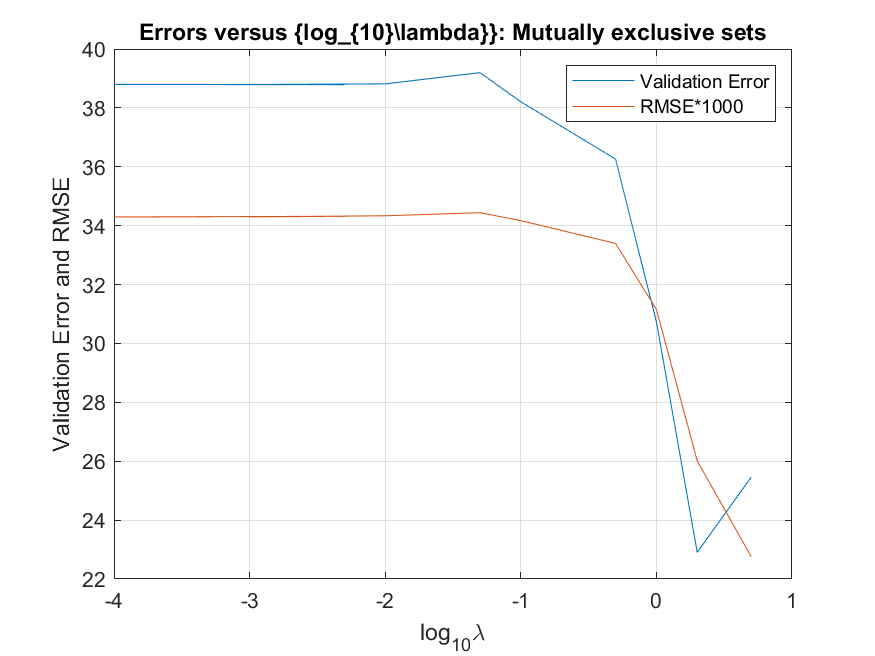
\includegraphics[width=0.7\linewidth]{images/plot1.png}
        \caption{Validation and RMSE errors(scale corrected) against $\Lambda$}
        \label{fig:1}
    \end{figure}
    We can see that the optimal values of $\lambda$ for both the plots come out to be the same and that the validation error plot approximates the RMSE plot quite closely. Given the fact that we don't know the RMSE beforehand since we don't even have the absolute truth \textbf{x}, we need a good proxy for the RMSE which the validation error apparently is. The validation and the RMSE errors decrease with increased lambda in general because we have progressively higher weight on having a sparser solution for \textbf{x}. 

    \item If the validation and the reconstruction sets are not disjoint but coincident sets, we will have lower validation errors than before because the training set is also being used for calculating the validation errors. Note that the cardinality of validation and reconstruction sets is kept the same as part 1. The validation error should however increase with $\lambda$ as the validation error would be directly proportional to $\lambda$ for $\mathbf{y_i}$'s in \textbf{V} as we minimized J(\textbf{x}). This is further supported by the plot in shown in Figure \ref{fig:2}.
    \begin{figure}[h!]
        \centering
        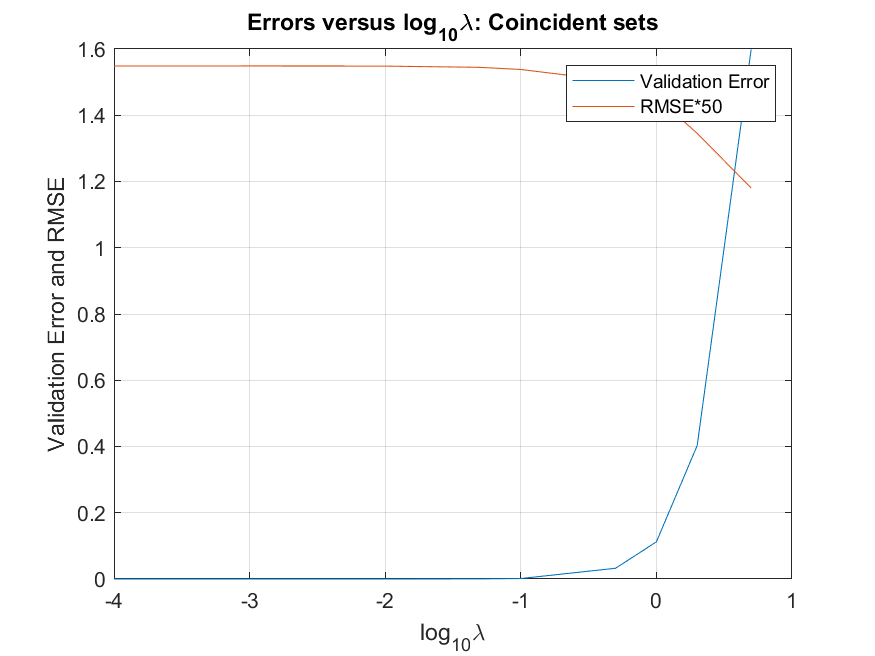
\includegraphics[width=0.7\linewidth]{images/plot2.png}
        \caption{Validation and RMSE errors(scale corrected) against $\Lambda$ for coincident validation and reconstruction sets}
        \label{fig:2}
    \end{figure}
    
    \item Theorem 3 from the paper \textbf{"On the Theoretical Analysis of Cross Validation In Compressive Sensing"} refers to the ability of the cross validation method to closely approximate the process of solving the optimization problem knowing the actual RMSE. Theorem 3 basically implies that the error using the CV(Cross Validation) method will be close enough to the oracle optimum error regardless of the sparsity of the solution we obtain after solving the optimization problem.\\
    We measure the extent to which the signal has been recovered by a parameter:
    \begin{gather*}
        \alpha^p\;:=\;\frac{||\mathbf{x}_{T\text{\textbackslash} T^p}||_2}{\sigma_n}
    \end{gather*}
    If $\alpha^p$ is large, then it implies that the probability that the cross validation error falls off with iterations is lower eventually implying that the corresponding recovered signal $\mathbf{x_{T^p}}$ cannot be an OMP-CV output. This measure is used when the sparsity of the recovered signal is not equal to that of the original signal. If it is equal and the indices of the sparse matrices match, then the recovery error is bounded by $\epsilon_g^0$ with a high probability where $\epsilon_g^0$ is the oracle optimum error. This implies that no matter what, the recovery error of OMP-CV is very close to the oracle optimum resulting in it being able to be used as a proxy for actual mean squared error as it is not available to us at the time of solving the optimization problem.
    
    \item The regularization parameter($\lambda_N$) used in the LASSO problem in the last assignment was as follows:
    \begin{gather}
        \lambda_N\;=\;2\sigma\sqrt{3\frac{log\left(\frac{ep}{k}\right)}{N}}
    \end{gather}
    We see here that we need the noise model's parameter(standard deviation here) and the sparsity of the actual result to actually optimize the solver by setting the optimum regularization parameter. Using the Cross-validation method for carrying out the iterations of the algorithm and for determining the optimum $\lambda$ is better here as it does not require any input from the user regarding the sparsity of the actual signal or the noise level parameters. The actual mean is inferred from the output of the algorithm on each iteration itself and is used to determine the number of the iterations to be carried out rather than relying on a static assignment of the regularization parameter.
\end{enumerate}



\clearpage
\item Consider that you learned a dictionary $\boldsymbol{D}$ to sparsely represent a certain class $\mathcal{S}$ of images - say handwritten alphabet or digit images. How will you convert $\boldsymbol{D}$ to another dictionary which will sparsely represent the following classes of images? Note that you are not allowed to learn the dictionary all over again, as it is time-consuming. 
\begin{enumerate}
\item Class $\mathcal{S}_1$ which consists of images obtained by applying a known derivative filter to the images in $\mathcal{S}$. 
\item Class $\mathcal{S}_2$ which consists of images obtained by rotating a subset of the images in class $\mathcal{S}$ by a known fixed angle $\alpha$, and the other subset by another known fixed angle $\beta$.
\item Class $\mathcal{S}_3$ which consists of images obtained by applying an intensity transformation $I^i_{new}(x,y) = \alpha (I^i_{old}(x,y))^2 + \beta (I^i_{old}(x,y)) + \gamma$ to the images in $\mathcal{S}$, where $\alpha,\beta,\gamma$ are known.  
\item Class $\mathcal{S}_4$ which consists of images obtained by applying a known blur kernel to the images in $\mathcal{S}$. 
\item Class $\mathcal{S}_5$ which consists of images obtained by applying a blur kernel which is known to be a linear combination of blur kernels belonging to a known set $\mathcal{B}$, to the images in $\mathcal{S}$. 
\item Class $\mathcal{S}_6$ which consists of 1D signals obtained by applying a Radon transform in a known angle $\theta$ to the images in $\mathcal{S}$. 
\item Class $\mathcal{S}_7$ which consists of images obtained by translating a subset of the images in class $\mathcal{S}$ by a known fixed offset $(x_1,y_1)$, and the other subset by another known fixed offset $(x_2,y_2)$. Assume appropriate zero-padding and increase in the size of the image canvas owing to the translation.
\textsf{[4+4+4+4+4+6+4=30 points]}
\end{enumerate}
\textbf{Sol:}\\
An image \textbf{I} is represented as a combination of dictionary atoms of the Dictionary matrix $\mathbf{D}\;=\;{\mathbf{d_1}|\mathbf{d_2}|\dots|\mathbf{d_k}}$ where \textbf{k} is the reduced dimensions of the dictionary coefficients \textbf{s}. The image \textbf{I} can therefore be written as follows:
\begin{gather}
    \mathbf{I}\;=\;\sum_{j=1}^Ss_j\mathbf{d_{m_j}}
\end{gather}
where $s_j$ are the dictionary coefficients and the $m_j$ are the column indices of the non-zero dictionary coefficients and S is the number of dictionary atoms that the image \textbf{I} uses. Reshaping the dictionary atoms into a matrix, we can observe that:
\begin{gather}
    I(x,y)\;=\;\sum_{j=1}^Sa_jd_{m_j}(x,y)\quad\forall(x,y)\in\mathbf{I}\\
    \implies f(I(x,y))\;=\;\sum_{j=1}^na_jI(x_j,y_j)\quad\forall(x,y)\in\mathbf{I}\nonumber\\
    \implies f(I(x,y))\;=\;\sum_{j=1}^na_j\left(\sum_{i=1}^Ss_id_{m_i}(x_i, y_i)\right)\nonumber\\
    \implies f(I(x,y))\;=\;\sum_{i=1}^Ss_i\left(\sum_{j=1}^na_jd_{m_i}(x_i, y_i)\right)\;=\;\sum_{i=1}^Ss_if(d_{m_i}(x, y))
    \label{eq:1}
\end{gather}
where $(x_j, y_j)$ are the pixels on which the linear function of $I(x,y)$ depends upon. 
From Eq. \ref{eq:1}, we get that a linear function operation on an image $\mathbf{I}$ is equivalent to a linear summation of a similar linear function on the dictionary atoms.
\begin{enumerate}
    \item Applying a derivative filter to an image is equivalent to performing a linear function on the image. The function can be a simple subtraction operation between adjacent pixel values. The new dictionary atoms need to also undergo the same linear operation and then be reshaped to be a column to form the new dictionary. The newly formed dictionary is  $\mathbf{D_1}\;=\;[f(\mathbf{d_1})\;|\;f(\mathbf{d_2})\;|\dots|\;f(\mathbf{d_k})]$ where the function f(.) applies the derivative function on the dictionary atoms reshaped to be of the image dimensions and then reshaped again to be a column which is then concatenated together to form a new Dictionary matrix $\mathbf{D_1}$.
    
    \item Rotation of an image can similarly be represented as a linear operation. Since the images are rotated by two different angles, we can't get away with only rotating the dictionary atoms by just a single angle. To have a sparsely represented dictionary representation of $\mathcal{S}_2$, we need to rotate the dictionary atoms with different angles $\alpha$ and $\beta$ and concatenate the two separate dictionaries like $\mathbf{D_2}\;=\;[\mathbf{D_\alpha}\;|\;\mathbf{D_\beta}]\;=\;[\mathbf{d_{\alpha_1}}\;|\dots|\mathbf{d_{\alpha_k}}\;|\;\mathbf{d_{\beta_1}}|\dots|\;\mathbf{d_{\beta_k}}]$.
    
    \item The new image can be represented mathematically as:
    \begin{gather}
        I(x,y)\;=\;\sum_{i=1}^Ss_id_{m_i}(x,y)\quad\forall(x,y)\in\mathbf{I}\nonumber\\
        \implies I_{new}(x,y)\;=\;\alpha\left(\sum_{i=1}^Ss_id_{m_i}(x,y)\right)^2\;+\;\beta\left(\sum_{i=1}^Ss_id_{m_i}(x,y)\right)\;+\;\gamma\nonumber\\
        \implies I_{new}(x,y)\;=\;\alpha\left(\sum_{i=1}^Ss_i^2d_{m_i}^2(x,y)\;+\;2\sum_{i\neq j}s_is_jd_{m_i}(x,y)d_{m_j}(x,y)\right)\;+\;\beta\left(\sum_{i=1}^Ss_id_{m_i}(x,y)\right)\;+\;\gamma
    \end{gather}
    The new image can therefore, be written as a linear combination of the squares of the dictionary atoms along with pairwise products of the atoms and the original dictionary itself i.e.
    \begin{gather*}
        \mathbf{D_{sq}}\;=\;[\mathbf{d_1^2}\;|\;\mathbf{d_2^2}\;|\dots|\;\mathbf{d_k^2}]\\
        \mathbf{D_{pair}}\;=\;[\mathbf{d_i}\cdot\mathbf{d_j}]\quad\forall i\neq j\\
        \mathbf{D_3}\;=\;[\mathbf{D_{sq}}\;|\;\mathbf{D_{pair}}\;|\;\mathbf{D}\;|\;\mathbf{1}]
    \end{gather*}
    where $\mathbf{d_i^2}$ is the column vector $\mathbf{d_i}$ with the elements squared and correspondingly $\mathbf{d_i}\cdot\mathbf{d_j}$ is the element-wise product of the two columns $\mathbf{d_i}$ and $\mathbf{d_j}$. $\mathbf{1}$ is a column vector with all the elements being 1. This models the constant $\gamma$. The new dictionary $\mathbf{D_3}$ is now able to model a sparse representation of the new class of images $\mathcal{S}_3$
    
    \item Applying a blur kernel to an image results in a linear transformation of pixels like the Gaussian blur filter which is just a linear summation of the surrounding pixels. So, if f(.) is a blur kernel function, we can apply it to the dictionary atoms as well and reshape it to a column and then concatenate to make the new dictionary just like we do in the first part for the derivative filter:
    \begin{gather*}
        \mathbf{D_4}\;=\;[f(\mathbf{d_1})\;|\;f(\mathbf{d_1})\;|\dots|\;f(\mathbf{d_k})]
    \end{gather*}
    
    \item The final blur kernel applied on an image from $\mathcal{S}$ can be easily represented as a linear representation of the individual blur kernels from the set $\mathcal{B}$ i.e. an image from $\mathcal{S}_5$ can be represented as:
    \begin{gather*}
        \mathbf{I_{new}}\;=\;\sum_{i=1}^Tc_ib_i(\mathbf{I})
    \end{gather*}
    where T is the number of blur kernels actually being combined for computing the blurred image and $c_i$ is the corresponding coefficient used for the $i^{th}$ blur kernel.\\
    So the new dictionary matrix can be made by including the linear transformation of each dictionary atom under each of the blur kernels as the final image is the linear combination of the transformed image under different blur kernels:
    \begin{gather*}
        \mathbf{D_5}\;=\;[\mathbf{b_1(D)}\;|\;\mathbf{b_2(D)}\;|\dots|\;\mathbf{b_T(D)}]
    \end{gather*}
    
    \item Since we have a fixed angle $\theta$ to calculate the radon transform along, we can get the discrete radon transform as follows:
    \begin{gather*}
        \mathcal{R}_\rho(\mathbf{I})\;=\;\sum_{x=0}^{M-1}\sum_{y=0}^{N-1}I(x,y)\delta(x\cos{\theta}+y\sin{\theta}-\rho)\\
        \implies \mathcal{R}_\rho(\mathbf{I})\;=\;\sum_{x=0}^{M-1}\sum_{y=0}^{N-1}\left(\sum_{i=1}^Ss_id_{m_i}(x,y)\right)\delta(x\cos{\theta}+y\sin{\theta}-\rho)\\
        \implies \mathcal{R}_\rho(\mathbf{I})\;=\;\sum_{i=1}^Ss_i\left(\sum_{x=0}^{M-1}\sum_{y=0}^{N-1}d_{m_i}(x,y)\delta(x\cos{\theta}+y\sin{\theta}-\rho)\right)\;=\;\sum_{i=1}^Ss_i\left(\mathcal{R}\rho(\mathbf{d_{m_i}})\right)\\
    \end{gather*}
    Here, we can see that the radon transform of an image can be represented as a linear combination of the radon transform of the corresponding dictionary atoms which can then be concatenated to form the new dictionary matrix $\mathbf{D_6}$:
    \begin{gather*}
        D_6\;=\;[\mathcal{R}\rho(\mathbf{d_1})\;|\;\mathcal{R}\rho(\mathbf{d_2})\;|\dots|\;\mathcal{R}\rho(\mathbf{d_k})]
    \end{gather*}
    
    \item The translated image $\mathbf{I_{new}}$ can be represented as follows:
    \begin{gather}
        \mathbf{I_{new}}(x,y)\;=\;\mathbf{I}(x-x_1,y-y_1)\quad\text{where}\\
        \mathbf{I}(x,y)\;=\;0\quad\forall x<0,\;y<0\nonumber\\
        \implies\mathbf{I_{new}}(x,y)\;=\;\mathbf{I}(x-x_1,y-y_1)\;=\;\sum_{i=1}^Ss_id_{m_i}(x-x_1,y-y_1)\;=\;\sum_{i=1}^Ss_if(d_{m_i}(x,y))
    \end{gather}
    Now since we are using 2 different translations, we need to make a new Dictionary matrix $\mathbf{D_7}$ using dictionary atoms with both translations:
    \begin{gather}
        \mathbf{D_7}\;=\;[\mathbf{D_{(x_1,y_1)}}\;|\;\mathbf{D_{(x_2,y_2)}}]\;=\;[\mathbf{d_{(x_1,y_1)_1)}}\;|\dots|\;\mathbf{d_{(x_1,y_1)_k}}\;|\;\mathbf{d_{(x_2,y_2)_1}}\;|\dots|\;\mathbf{d_{(x_2,y_2)_k}}]
    \end{gather}
    where $d_{{(x_1,y_1)}_1}$ is the first dictionary atom translated by $(x_1,y_1)$ with appropriate zero-padding, and then reshaped into a column. Zero-padding works here too as linear combination of 0 pixels is still 0 for the zero-padded translated image from $\mathcal{S}_7$.
\end{enumerate}


\clearpage
\item How will you solve for the minimum of the following objective functions: (1) $J(\boldsymbol{A_r}) = \|\boldsymbol{A}-\boldsymbol{A_r}\|^2_F$, where $\boldsymbol{A}$ is a known $m \times n$ matrix of rank greater than $r$, and $\boldsymbol{A_r}$ is a rank-$r$ matrix, where $r < m, r < n$. (2) $J(\boldsymbol{R}) = \|\boldsymbol{A}-\boldsymbol{R} \boldsymbol{B}\|^2_F$, where $\boldsymbol{A} \in \mathbb{R}^{n \times m}, \boldsymbol{B} \in \mathbb{R}^{n \times m}, \boldsymbol{R} \in \mathbb{R}^{n \times n}, m > n$ and $\boldsymbol{R}$ is constrained to be orthonormal. Note that $\boldsymbol{A}$ and $\boldsymbol{B}$ are both known. \\
In both cases, explain briefly any one situation in image processing where the solution to such an optimization problem is required. \textsf{[5+5+5+5=20 points]}\\
\textbf{Sol:}\\
\begin{enumerate}
    \item The objective function is;
    \begin{gather}
        J(\mathbf{A_r})\;=\;||\mathbf{A}-\mathbf{A_r}||^2_F
    \end{gather}
    Solving for $\mathbf{A_r}$ implies finding the best r-rank approximation of the matrix $\mathbf{A}$. We can do this by using the r-largest singular values and the corresponding eigenvectors from $\mathbf{U}$ and $\mathbf{V}$ to construct $\mathbf{A_r}$.\\
    Low-rank matrices can be used for modeling images of a convex Lambertian surface under various illuminations. This suits applications where we need to extract underlying information which has a lot of illumination variation, such as \textbf{background extraction}.
    
    \item The objective function is:
    \begin{gather}
        J(\mathbf{R})\;=\;||\mathbf{A}-\mathbf{RB}||_F^2\quad\text{where}
    \end{gather}
    $\mathbf{R}$  is an orthonormal matrix.
    \begin{gather*}
        min||\mathbf{A}-\mathbf{RB}||_F^2\;=\;min\left(Tr\left((\mathbf{A}-\mathbf{RB})^T(\mathbf{A}-\mathbf{RB})\right)\right)\;=\;min\left(Tr\left(\mathbf{A^TA}-2\mathbf{A^TRB}+\mathbf{B^TB}\right)\right)\\
        \implies min||\mathbf{A}-\mathbf{RB}||_F^2\;=\;max\left(Tr\left(\mathbf{A^TRB}\right)\right)\;=\;max\left(Tr\left(\mathbf{RBA^T}\right)\right)
    \end{gather*}
    Using SVD on $\mathbf{BA^T}\;=\;UDV^T$:
    \begin{gather*}
        min||\mathbf{A}-\mathbf{RB}||_F^2\;=\;max\left(Tr\left(\mathbf{RUDV^T}\right)\right)\;=\;max\left(Tr\left(\mathbf{V^TRUD}\right)\right)\;=\;max\left(Tr\left(\mathbf{Z(R)D}\right)\right)\\
        \implies min||\mathbf{A}-\mathbf{RB}||_F^2\;=\;max\left(\sum_iz_{ii}d_{ii}\right)\leq\sum_id_{ii}
    \end{gather*}
    which can be achieved when $\mathbf{Z(F)}\;=\;\mathbf{I}\;\implies\;\mathbf{R}\;=\;\mathbf{VU^T}$. This optimization problem is known as the \textbf{Orthogonal Procrustes} problem.\\
    We can use this optimization problem to solve for the rotation matrix $\mathbf{R}$ for \textbf{Tomography under unknown angles for 3D images} given the measured radon transforms and the input images. 
\end{enumerate}


\clearpage
\item We have studied the non-negative matrix factorization (NMF) technique in our course and examined applications in face recognition. I also described the application to hyperspectral unmixing. Your job is to find a research paper which explores an application of NMF in any task apart from these. You may look up the wikipedia article on this topic. Other interesting applications include stain normalization in pathology. Your job is to answer the following: (1) Mention the title, author list, venue and year of publication of the paper and include a link to it. (2) Which task does the paper apply NMF to? (3) How exactly does the paper solve the problem using NMF? What is the significance of the dictionary and the dictionary coefficients in solving the problem at hand? \textsf{[15 points]}\\

\textbf{Sol:} 
\begin{enumerate}

    \item \begin{itemize}
        \item Title: Email Surveillance Using Non-negative Matrix Factorization
        \item Author's List: MICHAEL W. BERRY, MURRAY BROWNE
        \item Venue: Computational \& Mathematical Organization Theory
        \item Publication:  14 January 2006 
        \item Link: \href{https://link.springer.com/article/10.1007/s10588-005-5380-5}{https://link.springer.com/article/10.1007/s10588-005-5380-5}
    \end{itemize}
    \item The paper applies NMF for the extraction and detection of concepts or
topics from electronic mail messages (Text mining). They use publicly released Enron electronic mail collection.
\item They encode sparse
term-by-message matrices and use a low rank non-negative matrix factorization algorithm to preserve natural data
non-negativity and avoid subtractive basis vector and encoding interactions present in techniques such as principal
component analysis\\

A collection of n messages indexed by m terms (or
keywords) can be represented as a m $ \times$ n term-by-message matrix X = [$x_{i j}$]. Each element or component $x_{ij}$ of the matrix X defines a weighted frequency at which term i occurs in message j. We approximate this 92,133 × 65,031 (sparse) matrix X via
\begin{gather*}
    X \approx WH = \sum_{k=1}^{50} W_kH^k
\end{gather*}
where W 92,133 × 50 are dictionary coefficients and H 50 × 65,031 is the dictionary. Both W and H are non negative as we use NMF. $W_k$ denotes the kth column of W, $H^k$ denotes the kth row of the matrix H, and r = 50 factors or parts are produced. Clearly, the non-negativity of W and H facilitate a parts-based representation of the matrix X whereby the basis (column) vectors of W or $W_k$ combine to approximate the original columns (messages) of the sparse matrix X. The outer product representation of W H in the above equation demonstrates how the rows of H or $H^k$ essentially specify the weights (scalar multiples) of each of the basis vectors needed for each of the 50 parts of the representation. The value of r depends on the data corpus.

\end{enumerate}

\clearpage
\item In parallel bean computed tomography, the projection measurements are represented as a single vector $\boldsymbol{y} \sim \textrm{Poisson}(I_o \exp(-\boldsymbol{R f}))$, where $\boldsymbol{y} \in \mathbb{R}^m$ with $m = $ number of projection angles $\times$ number of bins per angle; $I_o$ is the power of the incident X-Ray beam; $\boldsymbol{R}$ represents the Radon operator (effectively a $m \times n$ matrix) that computes the projections at the pre-specified known projection angles; and $\boldsymbol{f}$ represents the unknown signal (actually tissue density values) in $\mathbb{R}^n$. If $m < n$, write down a suitable objective function whose minimum would be a good estimate of $\boldsymbol{f}$ given $\boldsymbol{y}$ and $\boldsymbol{R}$ and which accounts for the Poisson noise in $\boldsymbol{y}$. State the motivation for each term in the objective function. Recall that if $z \sim \textrm{Poisson}(\lambda)$, then $P(z = k) = \lambda^k e^{-\lambda} / k!$ where $k$ is a non-negative integer. Now suppose that apart from Poisson noise, there was also iid additive Gaussian noise with mean 0 and known standard deviation $\sigma$, in $\boldsymbol{y}$. How would you solve this problem (eg: appropriate preprocessing or suitable change of objective function)?
\textsf{[6+ 4 = 10 points]}

\textbf{Sol:}
Given that y follows a poisson distribution,
\begin{gather*}
    y \sim \text{Poisson}(I_o exp(-Rf))\\
    \text{Where, } y\in R^m, f\in R^n, R \text{ is } m\times n \\
    y_i\sim \text{Poisson}(I_o exp(-R_if))\\
    \text{Where $R_i$ is the $i^{th}$ row of R}
\end{gather*}
For getting the suitable objective function, first we can say that the a good estimate of f would be that f that maximizes the following probability,
\begin{gather*}
   argmax_f\text{ } {P\left(\frac{y}{R, f}\right)} =  argmax_f\text{ } \prod_{i=0}^m P\left(\frac{y_i}{R, f}\right)\\
   \text{Which will also be same if we take the log, that is, a good estimate of f would be}\\
   argmax_f \text{ } \sum_{i=0}^m log\left(P\left(\frac{y_i}{R, f}\right)\right)\\
   \text{Now for a Poisson random variable z with parameter $\lambda$, the log probability will be}\\
   log(p(z=k)) = klog(\lambda) - \lambda - c (\text{constant independent of }\lambda )\\
   \text{Hence, ignoring the constant, and taking $\lambda = I_o exp(-R_if)$, the optimization problem becomes}\\
   argmax_f \text{ } \sum_{i=0}^m y_ilog(I_o exp(-R_if)) - I_o exp(-R_if)\\
   argmax_f \text{ } \sum_{i=0}^m y_ilog(I_o) + y_ilog(exp(-R_if)) - I_o exp(-R_if)\\
    \sum_{i=0}^m y_ilog(I_o) \text{ is independent of f}\\
    argmax_f \text{ } \sum_{i=0}^m -y_iR_if - I_o exp(-R_if)\\
    \text{Which is equivalent to}\\
    argmin_f \text{ } \sum_{i=0}^m y_iR_if + I_o exp(-R_if)
\end{gather*}
Hence, $\sum_{i=0}^m y_iR_if + I_o exp(-R_if)$ is the objective function whose argmin value will be a good approximation of f.\\

b) Given there is any additional gaussian noise with mean 0 and standard deviation $\sigma$. So, lets say the final output y is given by  y = y' + $\epsilon$,  $\epsilon \sim N(0, \sigma^2)$ and y' are the variable obtained by the sampling the poisson random variables as in part a. Again lets start from saying that a good estimate of f would the maximizes the probability, 
\begin{gather*}
    argmax_{f, \epsilon}\text{ } {P\left(\frac{y}{R, f}\right)} = argmax_{f, \epsilon}\text{ } {P\left(\frac{y'+\epsilon}{R, f}\right)} =  argmax_{f, \epsilon}\text{ } \prod_{i=0}^m P\left(\frac{y'_i}{R, f}\right)P_{\epsilon}(\epsilon_i)\\
    argmax_{f, y'}\text{ } \prod_{i=0}^m P\left(\frac{y'_i}{R, f}\right)P_{\epsilon}(y_i - y'_i)\\
    \text{Encoding the epsilon in $y'_i$ and taking } P_{\epsilon}(y_i - y'_i) = constant * exp(-\frac{(y_i - y'_i)^2}{2\sigma^2})\\
    \text{Taking logarithm, we know } log(exp(-\frac{(y_i - y'_i)^2}{2\sigma^2})) = -\frac{(y_i - y'_i)^2}{2\sigma^2}\\
    argmax_{f, y'}\text{ } \sum_{i=0}^m log(P\left(\frac{y'_i}{R, f}\right)) + \sum_{i=0}^m log( P_{\epsilon}(y_i - y'_i))\\
    \text{Using the solution from part a}\\
    argmax_{f, y'} \text{ } \sum_{i=0}^m -y'_iR_if - I_o exp(-R_if) -\frac{(y_i - y'_i)^2}{2\sigma^2}\\
    argmin_{f,y'} \text{ } \sum_{i=0}^m y'_iR_if + I_o exp(-R_if) +\frac{(y_i - y'_i)^2}{2\sigma^2}
\end{gather*}
Hence we need to change the objective function a little to solve for the case where y also consists a gaussian noise, The value of f that minimizes the above optimization problem will be a good estimate of the original f.


\end{enumerate}

\section*{Remarks}
The assignment folder for the code and other miscellaneous documents used to make this report is available \href{https://github.com/SKARA2000/CS754_HW4}{here}.
\end{document}